\chapter{Manual de uso de la interfaz}

En este apéndice construiremos un breve manual del uso de la interfaz: para visualizar las resonancias, interactuar con ella,  inferir con ella (clasificar o segmentar) y finalmente exportar una segmentación dada. Definiremos un flujo estándar del uso de la interfaz, aportando imágenes de su realización paso a paso.

\section{Diagrama de flujo de la interfaz}

A continuación, mostramos un diagrama de flujo correspondiente al uso estándar de la interfaz.

\begin{figure}[H]
	\centering
	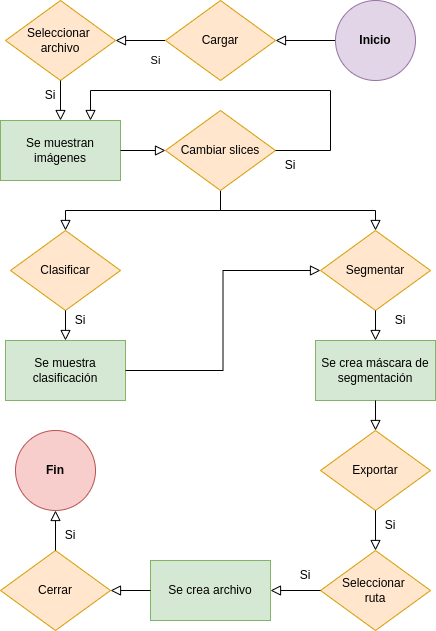
\includegraphics[width=0.4\linewidth]{imagenes/flujointerfaz.png}
	\caption{Diagrama de flujo de la interfaz.}
\end{figure}

\section{Tutorial sobre el flujo de la interfaz}

A continuación, veremos un tutorial del uso de la interfaz. Detallamos paso por paso cómo utilizarla. 

Al ejecutar la interfaz nos aparece la ventana principal que se muestra en la Figura C.2. Observamos tres bloques negros y uno blanco, los botones del uso de la interfaz y los selectores laterales para poder movernos en entre las imágenes.

\begin{figure}[H]
	\centering
	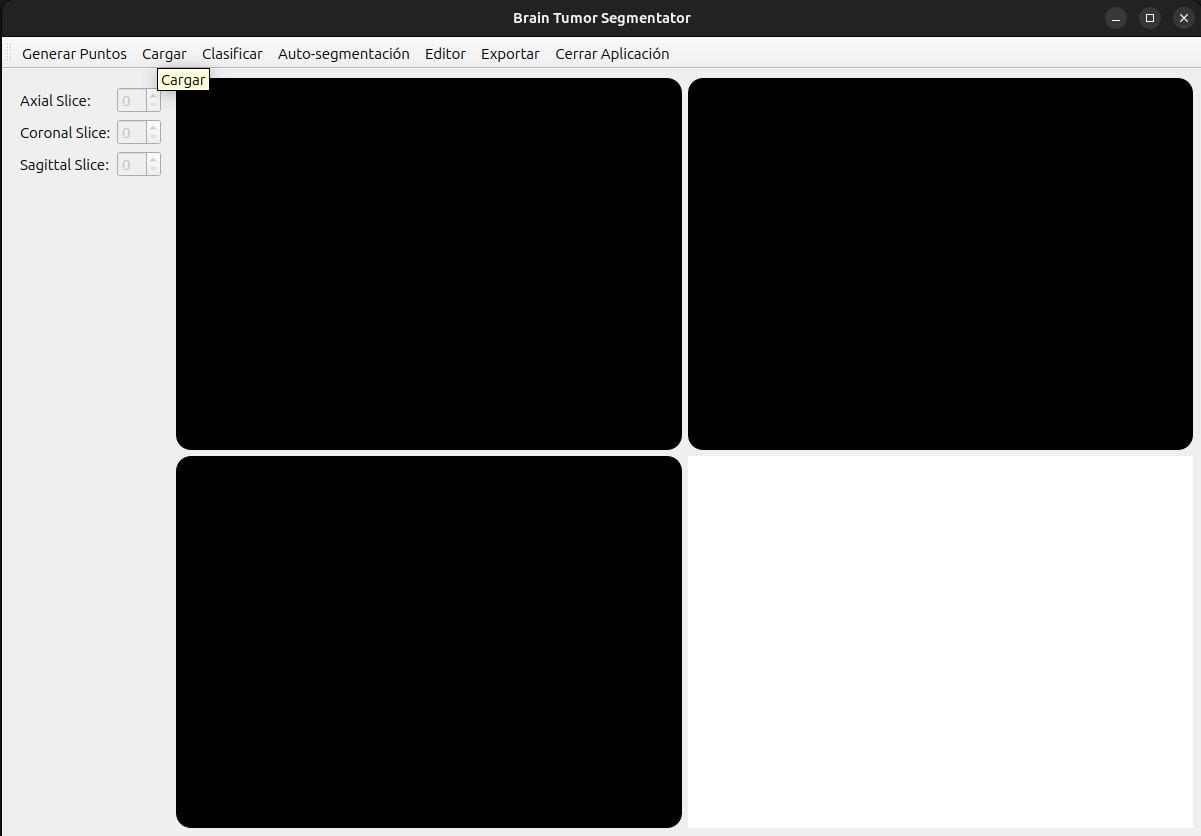
\includegraphics[width=0.7\linewidth]{imagenes/interfaz_inicio.png}
	\caption{Inicio de la interfaz.}
\end{figure}

Tras ello, debemos cargar alguna resonancia en nuestra carpeta de datos.

\begin{figure}[H]
	\centering
	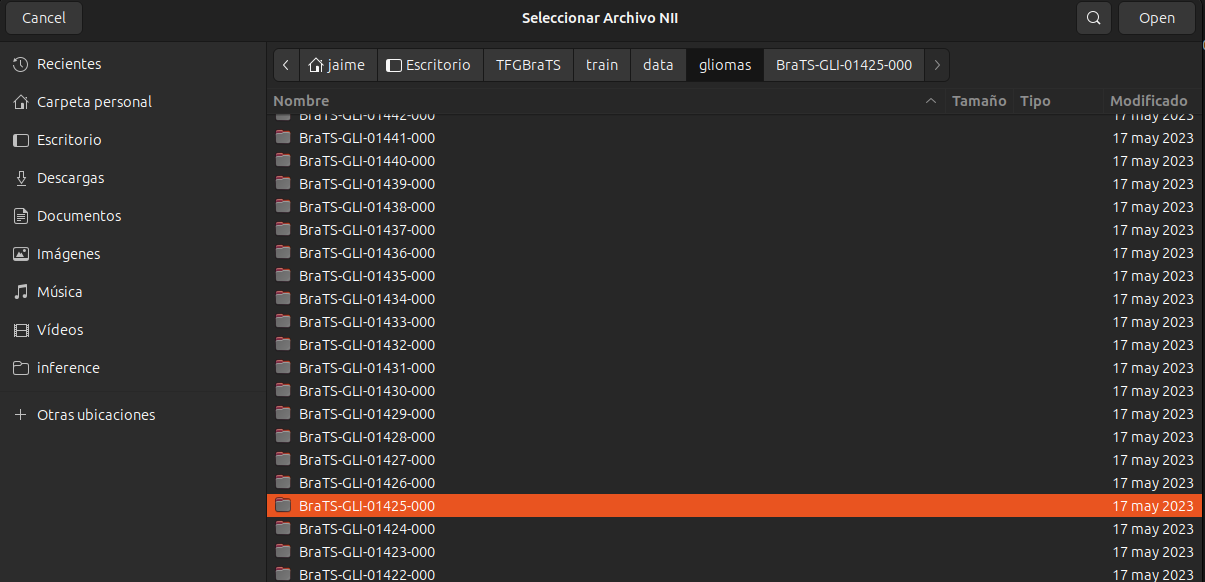
\includegraphics[width=0.7\linewidth]{imagenes/interfaz_seleccarchivo.png}
	\caption{Seleccionar archivo a cargar en la interfaz.}
\end{figure}

Por defecto, debemos escoger alguna prueba a visualizar (sólo se puede visualizar una prueba). Aunque selecciones sólo una prueba aquí cuando intentes inferir algo esto será indiferente ya que automáticamente seleccionará lo que necesite. 

\begin{figure}[H]
	\centering
	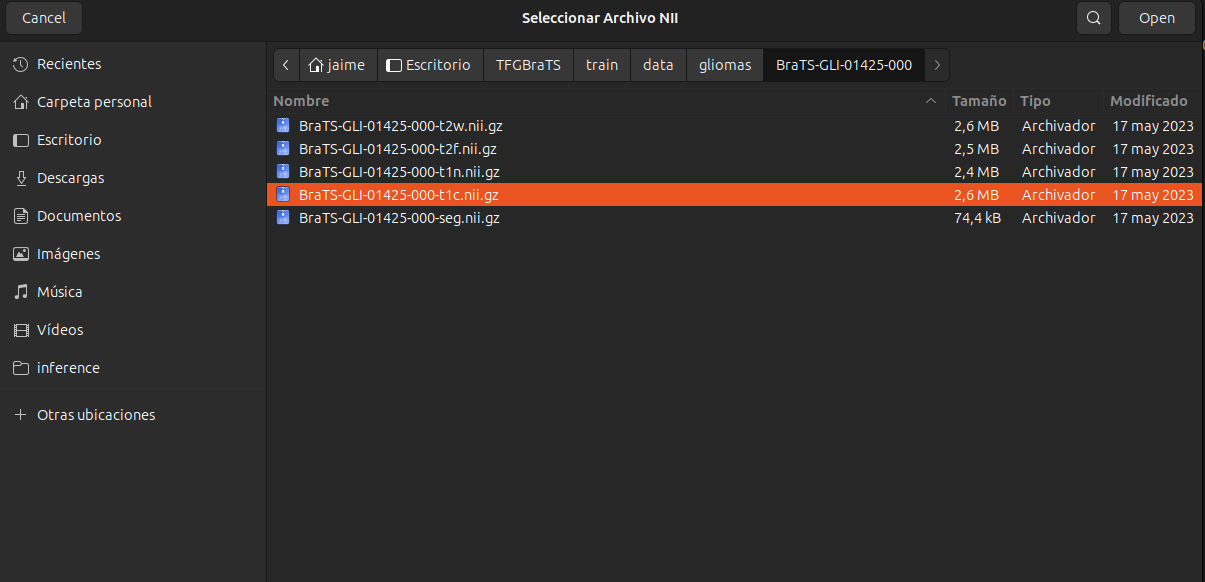
\includegraphics[width=0.7\linewidth]{imagenes/interfaz_seleccprueba.png}
	\caption{Seleccionar prueba a cargar en la interfaz.}
\end{figure}

En la Figura C.5. observamos como al abrir la prueba que queremos se nos cargan las imágenes y una reconstrucción 3D del cerebro como una nube de puntos. Podemos hacer clic con el ratón o movernos por la reconstrucción como deseemos.  Además observamos como ya los botones selectores de la derecha se habilitan, permitiendo poder recorrer el vector de imágenes de la resonancia para sus diferentes vistas.

\begin{figure}[H]
	\centering
	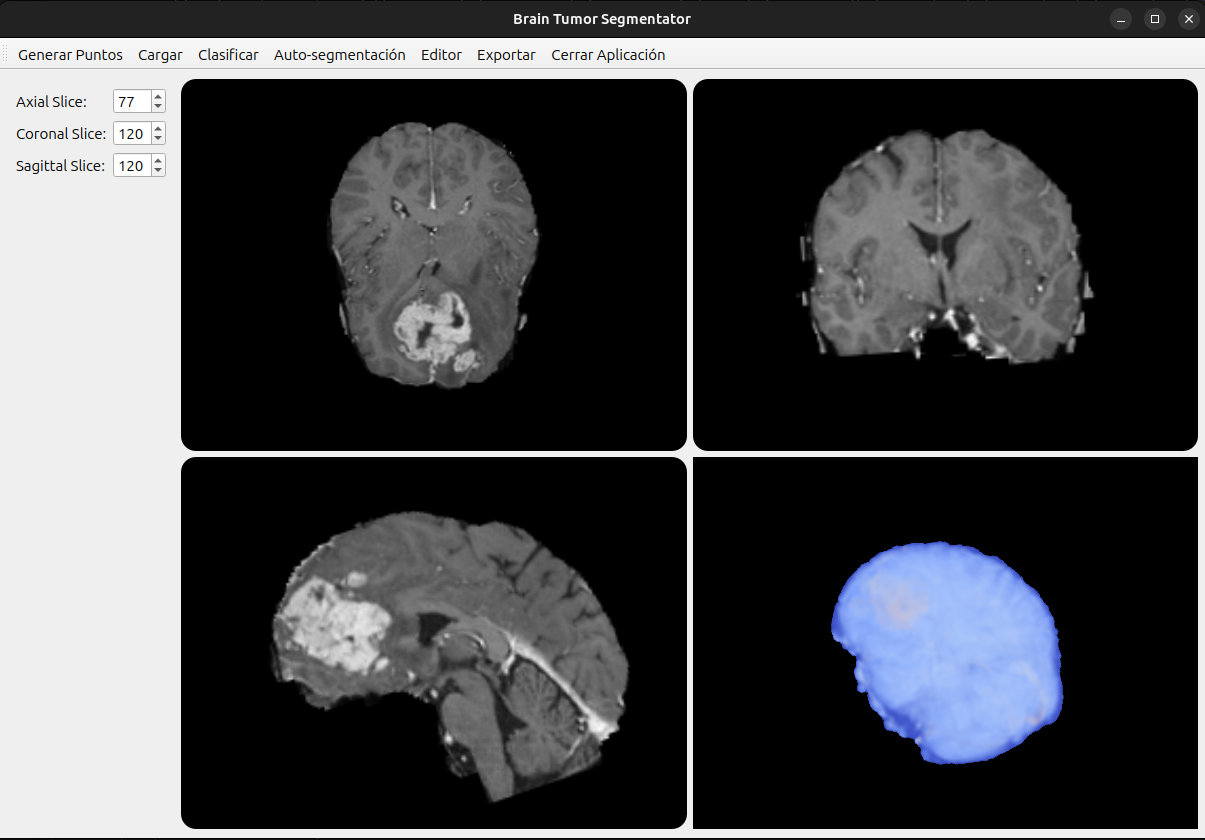
\includegraphics[width=0.7\linewidth]{imagenes/interfaz_visualizar.png}
	\caption{Visualizado de imágenes y 3D en la interfaz.}
\end{figure}

Para segmentar la imagen solo debemos darle al botón \textbf{Auto-Segmentación} tras ello la interfaz entiende que quieres inferir la máscara de segmentación de esa resonancia. Debemos esperar unos segundos, ya que es un proceso costoso.

\begin{figure}[H]
	\centering
	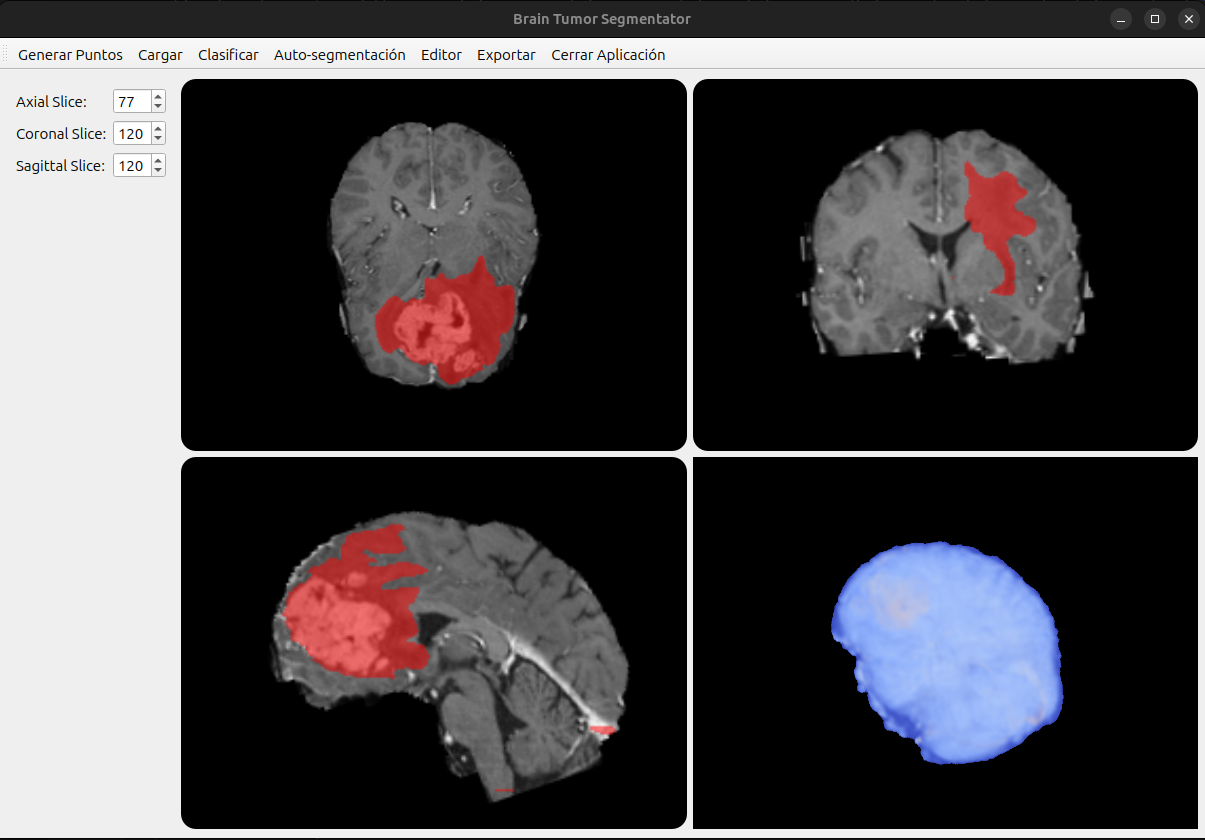
\includegraphics[width=0.7\linewidth]{imagenes/interfaz_mascara.png}
	\caption{Segmentar con la interfaz y visualizado de la máscara resultado.}
\end{figure}

En la Figura C.6, observamos como obtenemos la máscara de segmentación superponiéndose automáticamente a la imagen original. Esta máscara incluye la segmentación de todos los tejidos de la lesión tumoral.

Tras ello, podemos clasificar entre los dos tipos de tumores con la interfaz. Pulsamos el botón \textbf{Clasificar} y otra vez automáticamente entiende que quieres inferir la resonancia cargada.

\begin{figure}[H]
	\centering
	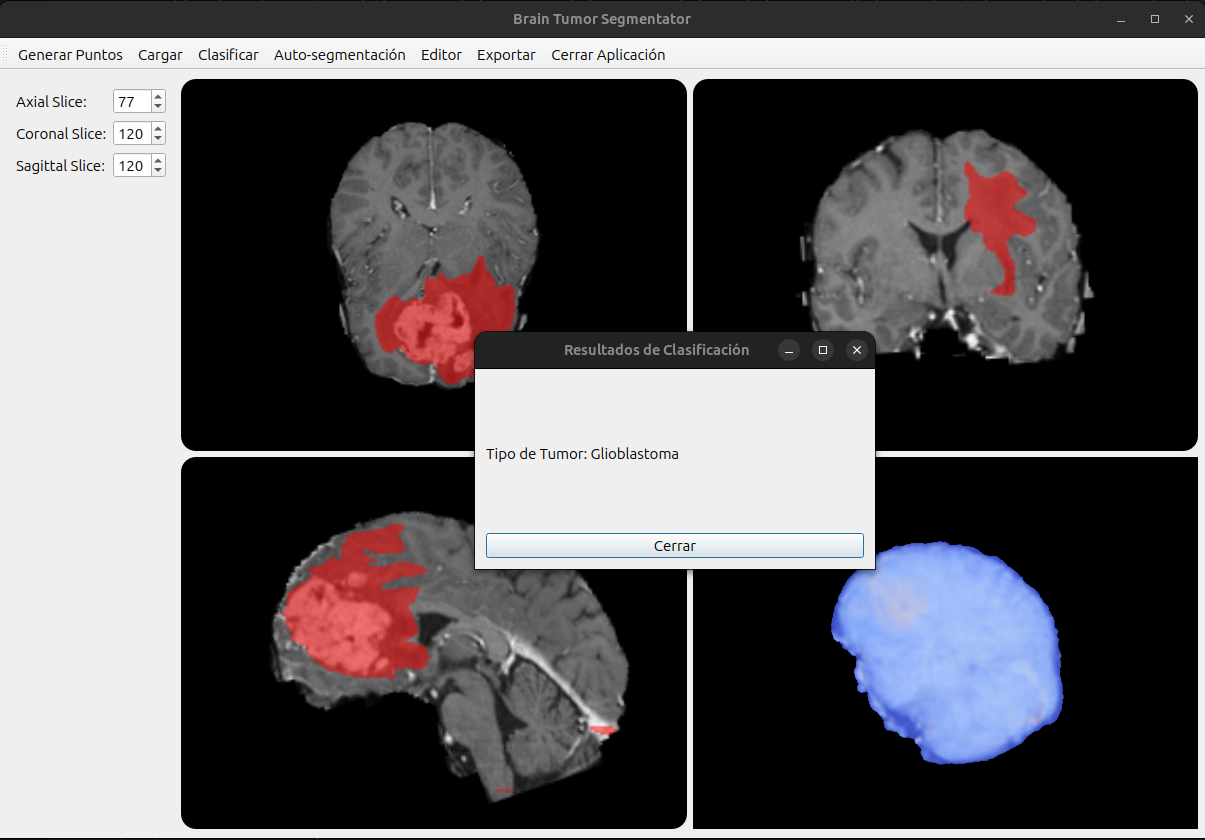
\includegraphics[width=0.7\linewidth]{imagenes/interfaz_clasificacion.png}
	\caption{Clasificar con la interfaz y resultados de clasificación.}
\end{figure}

En la figura C.7, observamos como tras pocos segundos aparece una pestaña emergente con los resultados del tipo de tumor.

Tras inferir ambos resultados, podemos exportar la máscara generada pulsando al botón \textbf{Exportar}. 

\begin{figure}[H]
	\centering
	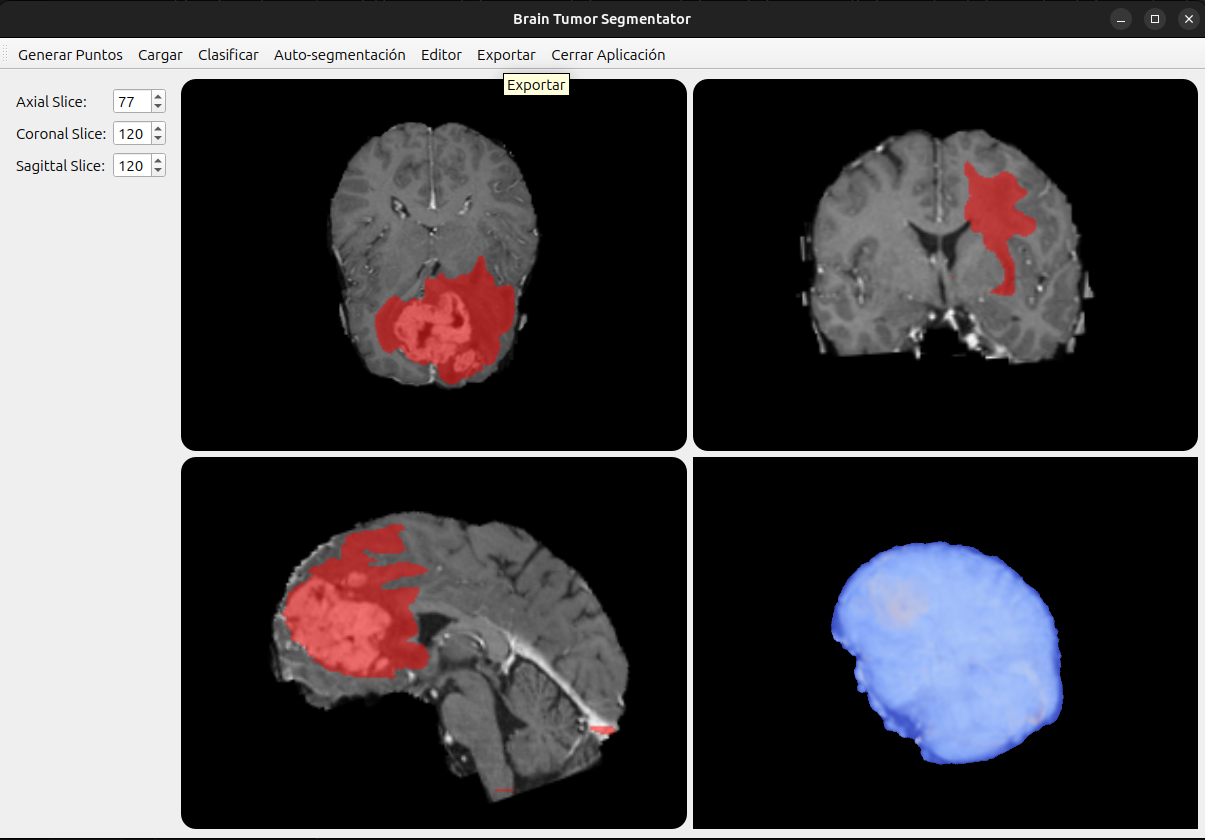
\includegraphics[width=0.7\linewidth]{imagenes/interfaz_exportar.png}
	\caption{Exportar segmentación con la interfaz.}
\end{figure}

Necesitamos guardarlo en alguna ruta que deseemos. Nos pregunta dónde guardarlo y con qué nombre. 

\begin{figure}[H]
	\centering
	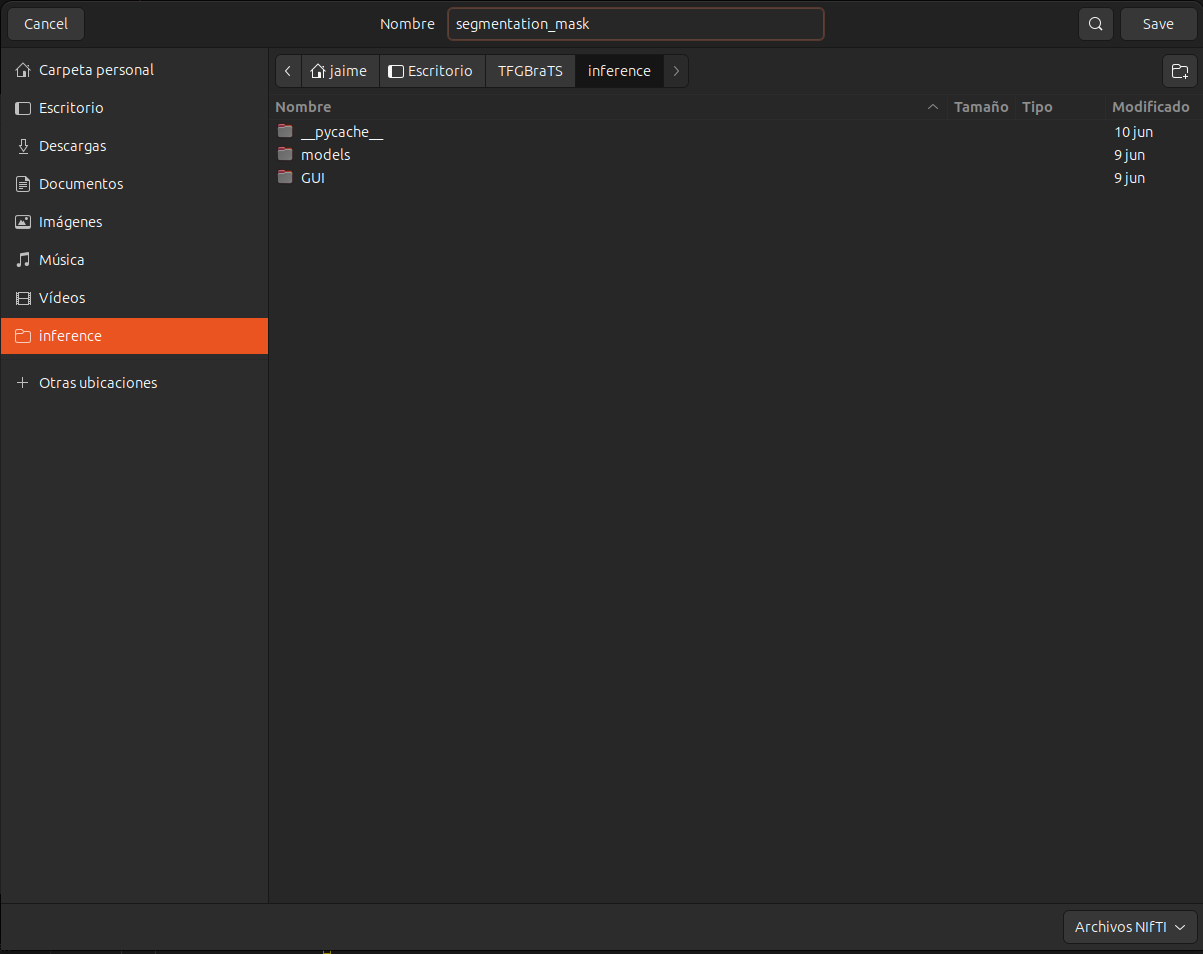
\includegraphics[width=0.7\linewidth]{imagenes/interfaz_seleccruta.png}
	\caption{Seleccionar ruta a exportar en la interfaz.}
\end{figure}

Si todo es correcto, nos dirá que fue correctamente guardado en una pestaña emergente. En caso contrario, también nos proporcionará el mensaje de error.

\begin{figure}[H]
	\centering
	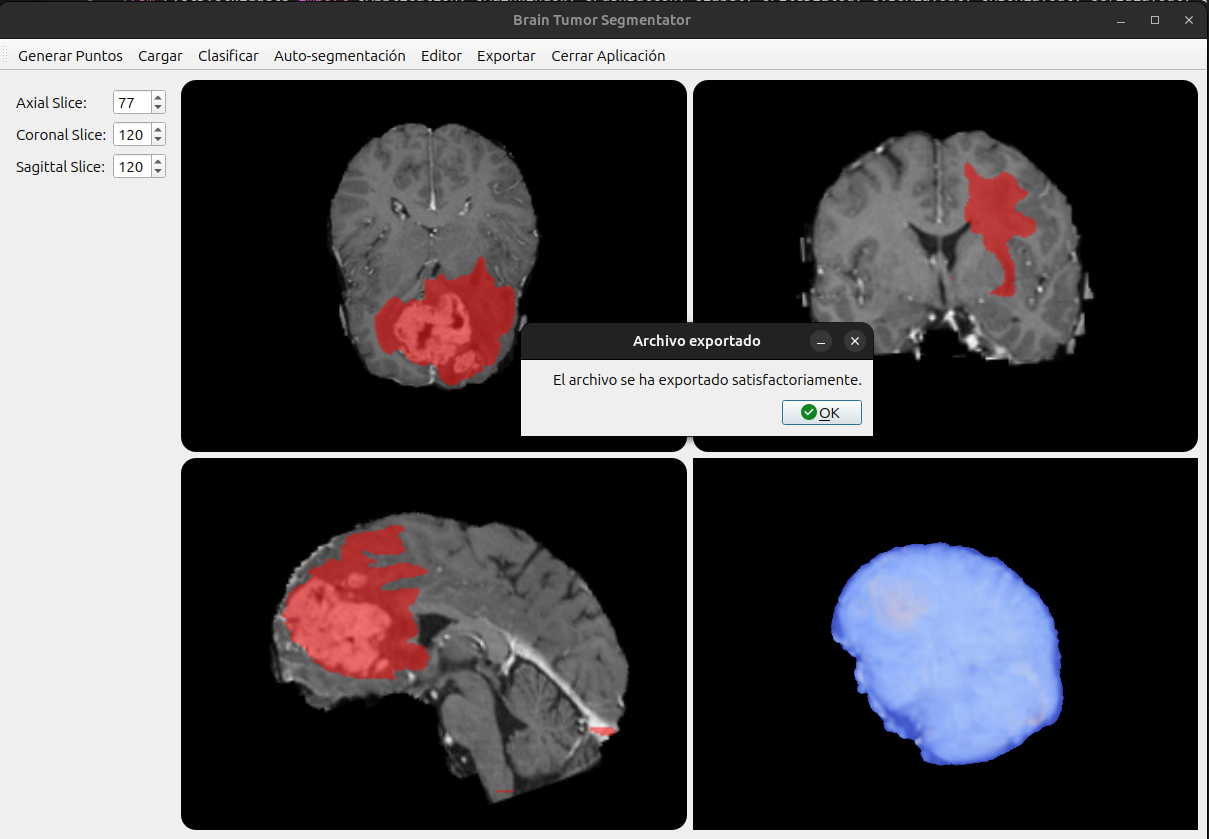
\includegraphics[width=0.7\linewidth]{imagenes/interfaz_mensaje.png}
	\caption{ Mensaje de exportación realizada correctamente.}
\end{figure}

Tras ello, podemos seguir infiriendo otras resonancias o cerrar la aplicación. Si cargamos otras resonancias el proceso es el mismo, la interfaz sobre escribirá los datos antiguos con los nuevos. Para cerrar correctamente la interfaz liberando explícitamente por el programa los recursos tan sólo pulsamos en \textbf{Cerrar Aplicación}.

